\documentclass{article}
\usepackage{graphicx}
\usepackage{amsmath}
\usepackage{mathtools}
\usepackage{amsfonts}
\usepackage{amssymb}
\usepackage{pdfpages}
\usepackage[]{mcode}
\renewcommand{\vec}[1]{\mathbf{#1}}

\begin{document}

\title{T-61.3050 Machine Learning: Basic Principles 
Solution of Prerequisite Knowledge Test 2013
}
\author{Md Mohsin Ali Khan(Student No: 336790)}

\maketitle


\begin{scriptsize}


\section{Algebra, Probabilities:}

\subsection*{a)}


First, assume another function $g:\Omega \rightarrow \mathbb{R}$. Now as per the definition of the operator $E$, we write:

\begin{eqnarray*}
E[f(\omega) + g(\omega)] &=& \sum_{\omega \in \Omega} P(\omega)(f(\omega)+g(\omega)) \\
&=& \sum_{\omega \in \Omega} P(\omega)f(\omega)+ P(\omega)g(\omega) \\
&=& \sum_{\omega \in \Omega} P(\omega)f(\omega)+ \sum_{\omega \in \Omega}P(\omega)g(\omega) \\
&=& E[f(\omega)] + E[g(\omega)]
\end{eqnarray*}

Second, assume that $t$ is a scalar, Now as per the definition of the operator $E$, we write:
\begin{eqnarray*}
E[tf(\omega)] &=& \sum_{\omega \in \Omega} P(\omega)(tf(\omega)) \\
&=& \sum_{\omega \in \Omega}tP(\omega)(f(\omega)) \\
&=& t\sum_{\omega \in \Omega} P(\omega)(f(\omega))\\
&=& tE[f(\omega)]
\end{eqnarray*}

So, we can colclude that $E[\cdot]$ is a linear operator


\subsection*{b)}
According to the definition of variance:
\begin{eqnarray*}
Var[f(\omega)] &=& E[(f(\omega) - E[f(\omega)])^2]\\
&=& E[f(\omega)^2 - 2f(\omega)E[f(\omega)] + E[f(\omega)]^2]\\
&=& E[f(\omega)^2] - E[2f(\omega)E[f(\omega)]] + E[E[f(\omega)]^2] \text{				//As $E[\cdot]$ is a linear operator}\\
&=& E[f(\omega)^2] - 2E[f(\omega)]E[f(\omega)] + E[f(\omega)]^2E[1] \text{				//$E[f(\omega)]$ is scalar value}\\
&=& E[f(\omega)^2] - E[2f(\omega)E[f(\omega)]] + E[f(\omega)]^2\sum_{\omega \in \Omega}P(\omega)\\
&=& E[f(\omega)^2] - 2E[f(\omega)]^2 + E[f(\omega)]^2 \text{				//It is given that $\sum_{\omega \in \Omega}P(\omega) = 1$ }\\
&=& E[f(\omega)^2] - E[f(\omega)]^2
\end{eqnarray*}


\section{Matrix Calculus:}

It is given that,
\begin{equation}
\vec{B} = \sum_{i=1}^n \lambda_i\vec{v}_i{\vec{v}_i}^T
\end{equation}

Multiplying both side of (1) by $\vec{v}_j$ where $j \in 1 \dotso n$, we can write


\begin{eqnarray*}
\vec{B}\vec{v}_j &=& \left(\sum_{i=1}^n \lambda_i\vec{v}_i{\vec{v}_i}^T\right)\vec{v}_j\\
\vec{B}\vec{v}_j &=& (\lambda_1\vec{v}_1{\vec{v}_1}^T + \lambda_2\vec{v}_2{\vec{v}_2}^T+\dotso + \lambda_n\vec{v}_n{\vec{v}_n}^T)\vec{v}_j\\
\vec{B}\vec{v}_j &=& \lambda_1\vec{v}_1{\vec{v}_1}^T\vec{v}_j +  \lambda_2\vec{v}_2{\vec{v}_2}^T\vec{v}_j+ \dotso + \lambda_j\vec{v}_j{\vec{v}_j}^T\vec{v}_j + \dotso + \lambda_n\vec{v}_n{\vec{v}_n}^T\vec{v}_j\\
\vec{B}\vec{v}_j &=& \lambda_j\vec{v}_j{\vec{v}_j}^T\vec{v}_j \text{	//As ${\vec{v}_i}^T\vec{v}_j=\delta_{i,j}$ where $\delta_{i,j} = 1$ when $i = j$ and $\delta_{i,j} = 0$ when $i \neq j$ )}\\
\vec{B}\vec{v}_j &=& \lambda_j\vec{v}_j
\end{eqnarray*}

So it is clear that $\lambda_j$ and $\vec{v}_j$ are Eigenvalues and Eigenvectors of the matrix $\vec{B}$



\section{Algorithms:}
\subsection*{The Algorithm:}
GenFibonacciuptoN($n$)\linebreak
Begin
\begin{itemize}
\item[1.] Declare an Array $Fib[1 .. n]$
\item[2.] $Fib[1] = 1, Fib[2] = 1$
\item[3.] For each $i \in \mathbb{N}$ starting from $3$ to $n$ in ascending order, do
\item[] 	i) $Fib[i]$ = $Fib[i-2]+Fib[i-1]$
\item[4.] Return the array $Fib[1 .. n]$. The $i$-th index holds the $i$-th Fibonacci Number
\end{itemize}
End\linebreak
	
\subsection*{Time Complexity:}
\begin{itemize}

\item[1] Worst case time complexity is: $T(n) = n-2$ i.e. $T(n) = O(n)$
\item[2] The algorithm has linear time complexity with the growth of input size
\end{itemize}


\section{Basic Data Analysis, Software Tools:}
\subsection*{Matlab Code:}


\begin{lstlisting}
fid = fopen('T-61_3050_data_set.txt');
A = fscanf(fid, '%f %f %f %f %f %f %f %f %f %f %f %f %f %f %f %f', [16 inf]);
fclose(fid);

A = A';

x = [0 0 0 0 0 0 0 0 0 0 0 0 0 0 0 0];
xsquare = [0 0 0 0 0 0 0 0 0 0 0 0 0 0 0 0];
xvar = [0 0 0 0 0 0 0 0 0 0 0 0 0 0 0 0];
max = 0;
secondmax = 0;
maxi = 0;
secondmaxi = 0;

for i=1:16,
    for j=1:4000
        x(i) = x(i) + A(j,i);
        xsquare(i) = xsquare(i) + A(j,i)^2;
    end
xvar(i) = xsquare(i)/4000 - (x(i)/4000)^2;
if xvar(i) > max
    secondmax = max;
    secondmaxi = maxi;
    max = xvar(i);
    maxi = i;
end
end

maxvariancecolumn = A(:,maxi);
secondmaxvariancecolumn = A(:,secondmaxi);

plot(secondmaxvariancecolumn,maxvariancecolumn,'o');
\end{lstlisting}


\subsection*{Scatterplot of the the columns having largest variance:}
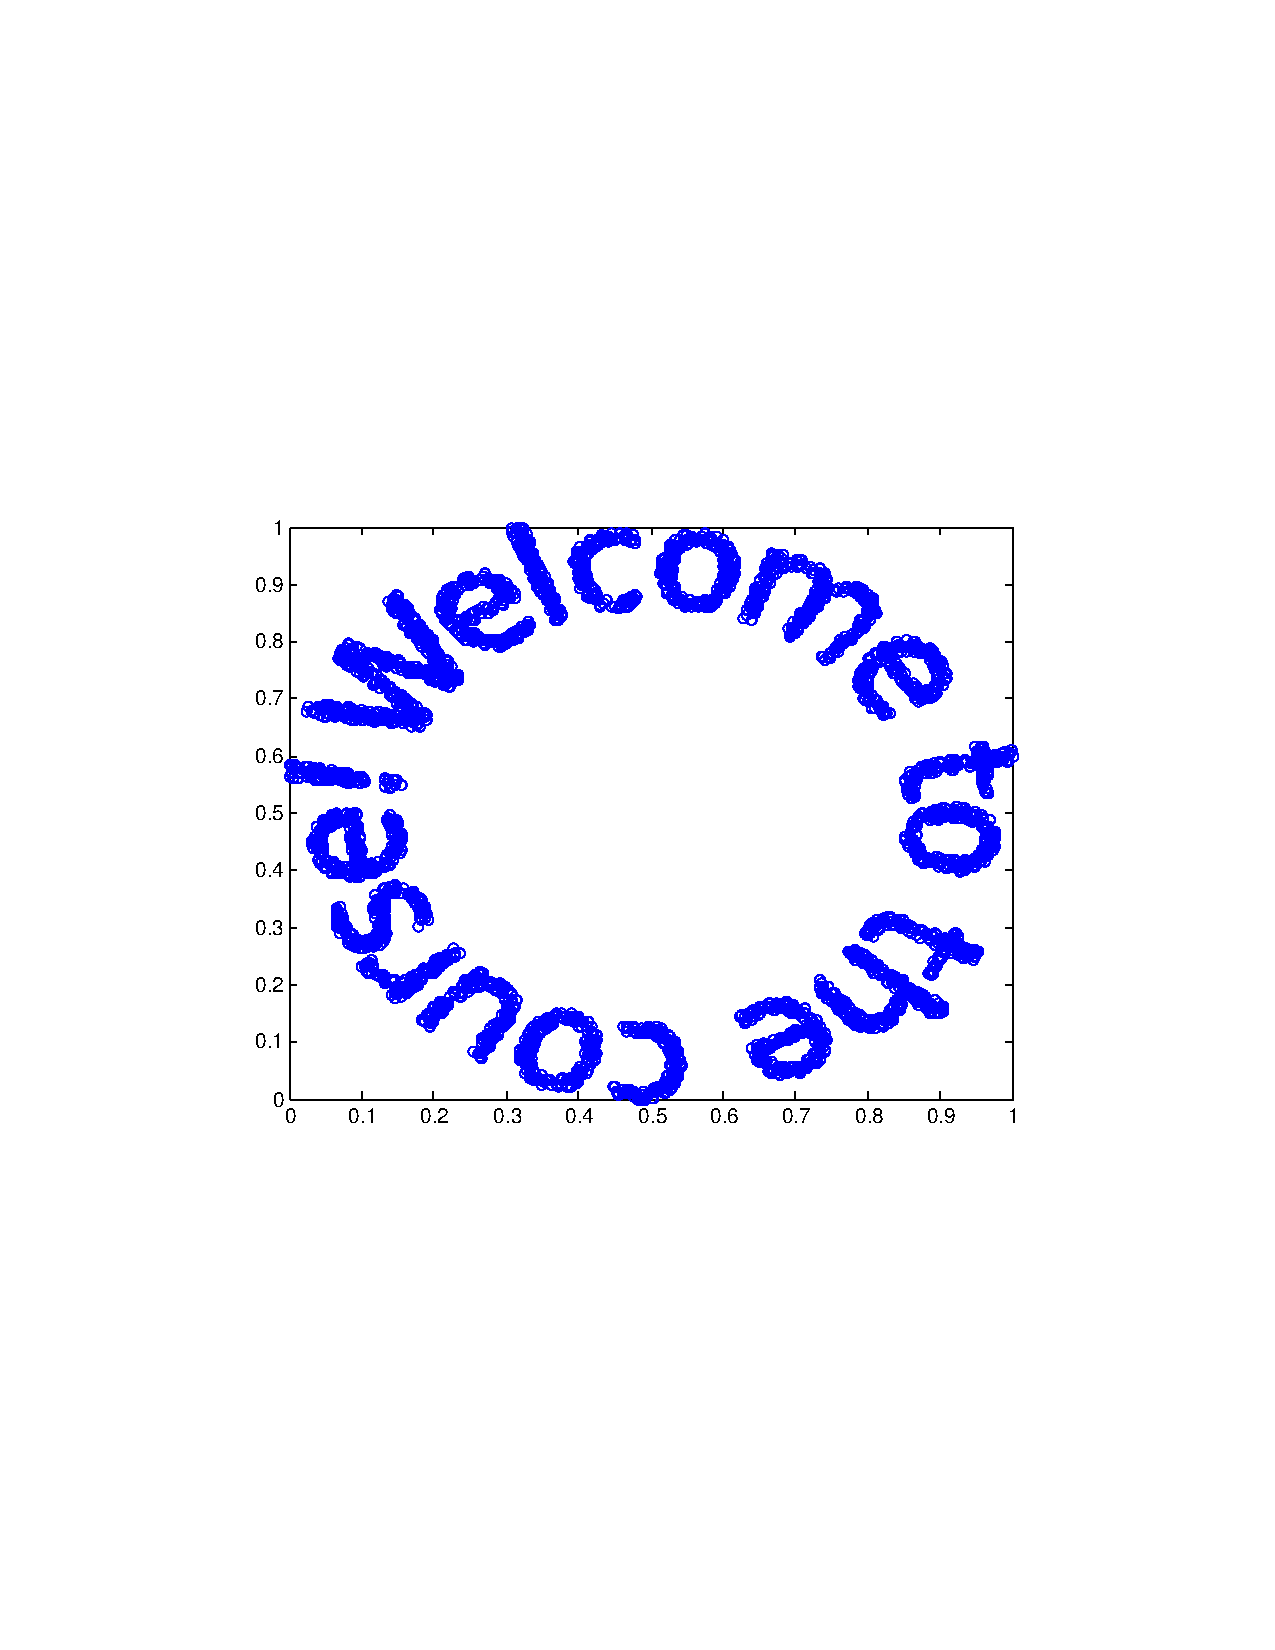
\includepdf[pages={1}]{scatterplot.pdf}





\end{scriptsize}

\end{document}